\PassOptionsToPackage{unicode=true}{hyperref} % options for packages loaded elsewhere
\PassOptionsToPackage{hyphens}{url}
%
\documentclass[]{article}
\usepackage{lmodern}
\usepackage{amssymb,amsmath}
\usepackage{ifxetex,ifluatex}
\usepackage{fixltx2e} % provides \textsubscript
\ifnum 0\ifxetex 1\fi\ifluatex 1\fi=0 % if pdftex
  \usepackage[T1]{fontenc}
  \usepackage[utf8]{inputenc}
  \usepackage{textcomp} % provides euro and other symbols
\else % if luatex or xelatex
  \usepackage{unicode-math}
  \defaultfontfeatures{Ligatures=TeX,Scale=MatchLowercase}
\fi
% use upquote if available, for straight quotes in verbatim environments
\IfFileExists{upquote.sty}{\usepackage{upquote}}{}
% use microtype if available
\IfFileExists{microtype.sty}{%
\usepackage[]{microtype}
\UseMicrotypeSet[protrusion]{basicmath} % disable protrusion for tt fonts
}{}
\IfFileExists{parskip.sty}{%
\usepackage{parskip}
}{% else
\setlength{\parindent}{0pt}
\setlength{\parskip}{6pt plus 2pt minus 1pt}
}
\usepackage{hyperref}
\hypersetup{
            pdftitle={Senior Project Report},
            pdfauthor={Samuel Helms},
            pdfborder={0 0 0},
            breaklinks=true}
\urlstyle{same}  % don't use monospace font for urls
\usepackage{longtable,booktabs}
% Fix footnotes in tables (requires footnote package)
\IfFileExists{footnote.sty}{\usepackage{footnote}\makesavenoteenv{longtable}}{}
\usepackage{graphicx,grffile}
\makeatletter
\def\maxwidth{\ifdim\Gin@nat@width>\linewidth\linewidth\else\Gin@nat@width\fi}
\def\maxheight{\ifdim\Gin@nat@height>\textheight\textheight\else\Gin@nat@height\fi}
\makeatother
% Scale images if necessary, so that they will not overflow the page
% margins by default, and it is still possible to overwrite the defaults
% using explicit options in \includegraphics[width, height, ...]{}
\setkeys{Gin}{width=\maxwidth,height=\maxheight,keepaspectratio}
\setlength{\emergencystretch}{3em}  % prevent overfull lines
\providecommand{\tightlist}{%
  \setlength{\itemsep}{0pt}\setlength{\parskip}{0pt}}
\setcounter{secnumdepth}{0}
% Redefines (sub)paragraphs to behave more like sections
\ifx\paragraph\undefined\else
\let\oldparagraph\paragraph
\renewcommand{\paragraph}[1]{\oldparagraph{#1}\mbox{}}
\fi
\ifx\subparagraph\undefined\else
\let\oldsubparagraph\subparagraph
\renewcommand{\subparagraph}[1]{\oldsubparagraph{#1}\mbox{}}
\fi

% set default figure placement to htbp
\makeatletter
\def\fps@figure{htbp}
\makeatother


\title{Senior Project Report}
\author{Samuel Helms}
\date{Advised by John Lafferty}

\begin{document}
\maketitle

{
\setcounter{tocdepth}{3}
\tableofcontents
}
\hypertarget{intro}{%
\section{Intro}\label{intro}}

\hypertarget{motivation}{%
\subsection{Motivation}\label{motivation}}

Word and sentence embeddings are an incredibly powerful tool for natural
language processing. Google Translate's error rate decreased by over
50\% when it switched to a model that used embeddings for translations
{[}(``A Neural Network for Machine Translation, at Production Scale''
n.d.).

The options for telling how good embeddings are before running them
through a downstream task like Google Translate are less amazing,
however: Researchers only have a few small datasets, which are largely
based on linguistic survey data, for this task (Schnabel et al. 2015).

One of the reason so few datasets for evaluating embeddings exist are
difficulties in determining when two words or sentences are different or
similar. Consider how difficult it is for a machine learning model to
determine that the phrase ``the red-faced man'' can be equivalent to
``the embarrassed man'' in the right context.

Mathematics is a type of language without this type of ambiguity about
whether two clauses mean the same thing. The equals sign tells us with
certainty when two expressions are equivalent to each other. Therefore
mathematics is a perfect test bed for new embeddings models, since every
mathematics text contains tens or hundreds of equivalencies with which
to evaluate embeddings.

As far as I am aware, no one has yet taken advantage of the equals sign
for creating and evaluating embeddings. Throughout the course of this
semester, I have created the first ever dataset of equivalent equations.

\hypertarget{applications}{%
\subsection{Applications}\label{applications}}

This project will enable researchers and data scientists who work with
mathematics texts to evaluate the intrinsic success of their embeddings.
It may also enable better understanding of embedding in general. If I am
able to create a large enough dataset of equivalent equations, the
equivalent equations could also be used to train embeddings in a
supervised fashion.

\hypertarget{background}{%
\subsection{Background}\label{background}}

This fall, I started working with a research group that Prof.~John
Lafferty helped found called
\href{https://github.com/hopper-project}{The Hopper Project}. The Hopper
Project has created a dataset of academic articles from arxiv and coded
up a pipeline that extracts LaTeX from these academic articles. I will
extract equivalent equations from this dataset.

\hypertarget{outcome-what-ive-actually-created}{%
\subsection{Outcome: What I've Actually
Created}\label{outcome-what-ive-actually-created}}

\hypertarget{a-dataset-of-equations-related-by-things-like-equals-signs}{%
\subsubsection{A dataset of equations related by things like equals
signs}\label{a-dataset-of-equations-related-by-things-like-equals-signs}}

You can get a premade dataset of with 5 million equations in it at
\url{https://github.com/samghelms/similar_eqs_senior_proj}, in the
\texttt{all\_eqs} folder. This is a folder of files with processed
equations. The repository includes examples on how to read in and work
with these files, and instructions on how to generate your own dataset
of interesting equation pairs.

These equations can be useful for a myriad of tasks, such as evaluating
embeddings -- pairs split by relations should be equivalent in some
sense -- or training embeddings models themselves. The final dataset has
millions of equations, so the data can easily be used for such a task.

\hypertarget{a-set-of-scripts-for-tokenizing-tex-and-identifying-useful-equations}{%
\subsubsection{A set of scripts for tokenizing TeX and identifying
useful
equations}\label{a-set-of-scripts-for-tokenizing-tex-and-identifying-useful-equations}}

If you're reading this report on github, you probably already know this.

The repository at
\url{https://github.com/samghelms/similar_eqs_senior_proj} contains the
library of scripts and instructions on how to use them, as well as a
premade pipeline for processing TeX formulas. Every function is unit
tested and has been reworked many times based on feedback from Hopper
Project researchers and mistakes made in processing jobs.

\hypertarget{a-suite-of-tools-for-working-with-equation-embeddings}{%
\subsubsection{A suite of tools for working with equation
embeddings}\label{a-suite-of-tools-for-working-with-equation-embeddings}}

Equations texts are harder to work with than normal english texts
because they are written in LaTeX. I started working on a set of tools
for visualizing mathematics in embeddings models this fall (Helms 2017).

This evolved into seeing how I contribute and work within existing
tools. I've since come up with ways of rendering rich html/javascript
representations of math in jupyter notebooks, and I have made a gist
showing how to do so available to the public:
\href{https://gist.github.com/samghelms/d1bd0a941c29044d6baa213ad96daa67}{https://github.com/samghelms/similar\_eqs\_senior\_proj}.

I also got interested in being able to visualize math on T-SNE plots
(for the uninitiated: a 2d scatter plot that approximates high
dimensional vectors). I'm currently developing a fully fledged library
that allows you to easily create such plots, and you can see my
prototype in action here:
\url{https://samghelms.github.io/webgl-scatter/} (zoom in and hover!).

\hypertarget{the-code}{%
\section{The Code}\label{the-code}}

In this section, I will go over the code I have written to tokenize TeX
equations at a high level and explain why I wrote it the way I did. Note
that this is only a high level discussion: look to the readme and
comments in the code base for specific instructions on how to use the
pipeline. Before I jump into the specifics of the code, I will give a
brief background on TeX to make it clearer why I had to go to the
lengths I did to get aligned few math equations.

Identifying and using equal equations in machine learning models
requires two things: One, being able to properly identify tokens (so
that the LaTeX code \texttt{\textbackslash{}\textbackslash{}int} is
treated as an atomic unit and not a sequence of the characters
``\textbackslash{}'', ``i'', ``n'', and ``t''); Two, being able to say
whether a subexpression is substantive enough to use in the model.

You could determine substantiveness (the second requirement) by doing
things like setting a string length cutoff for the subexpression and
taking tf-idf scores between two expressions on either side of an
equals, but this provides no guarantee of substantiveness--the
expression \texttt{x\ +\ y} is arguably just as substantive as
\texttt{\textbackslash{}\textbackslash{}frac\ \{\ x\_7\ \}\ \{\ y\_i\ \}},
with one operator and two variables, but it would be hard to determine
so based on tf-idf score or the length of the expression.

As a result of this difficulty in determining substantiveness, I decided
to implement a heuristic function that would make a shallow parse of the
TeX expression and determine if it contained at least one operator and
two variables and/or numbers at a high level. I arbitrarily decided on
this cutoff for the number of variables and expressions, and wrote the
code so this could be adjusted. By ``high level'' I mean not within a
subexpression or exponent, or a function argument--so f(x + y) would not
count as a substantive expression.

\hypertarget{a-brief-history-of-tex}{%
\subsection{A brief history of TeX}\label{a-brief-history-of-tex}}

You might be wondering why tokenization and parsing similar equations
was hard enough a task to spend a whole semester doing it. You would be
right to wonder: it should not be very hard to do, if not for the fact
that the core layout algorithms for TeX are all written in a virtually
extinct language called \href{https://en.wikipedia.org/wiki/WEB}{WEB}
written by the creator of TeX, Donald Knuth, himself.

Because WEB has been all but forgotten, the core TeX algorithms
implemented in it by Knuth are automatically cross-compiled into C code
before being used by TeX tools like texlive. This makes it extremely
difficult to hack into TeX's parsing algorithms and access their
internal data structures. Without access to the TeX algorithms or
internal data structures (or even source code that is easy to navigate
and/or understand), it is hard to even tokenize LaTeX codes, not to
mention parse them.

As a result, I have written my own tokenization function. I have not
written a complete TeX parser, but I have implemented a shallow parse
that can skip along the highest level of TeX code and check if it
contains certain types of operations.

A group at Harvard wrote a wrapper around KaTeX for tokenizing LaTeX
math expressions. I decided to write my own so that I could be
absolutely certain about the assumptions underlying the data and avoid
accidentally introducing bias into the data.

\hypertarget{tokenization}{%
\subsection{Tokenization}\label{tokenization}}

I implemented a finite state machine to tokenize TeX codes. It takes a
stream of characters from an equation from an arxiv text as input and
iterates over it, changing state with each new character. Depending on
the state and the character, the FSM will build a token or create a new
one.

The following input string will be tokenized to the following list by
the function \texttt{tokenize} in \texttt{tok.py}:

\texttt{\textquotesingle{}\textbackslash{}\textbackslash{}frac\{x\}\ \{y\}\ \textbackslash{}\textbackslash{}begin\{eq\ \}x\ =\ \textbackslash{}\textbackslash{}textfadfsad\{tets\}\ \textbackslash{}\textbackslash{}int\ 1.0\ .6\ \textbackslash{}\textbackslash{}end\{test\}\textquotesingle{}}

\texttt{{[}\textquotesingle{}\textbackslash{}\textbackslash{}frac\textquotesingle{},\ \textquotesingle{}\{\textquotesingle{},\ \textquotesingle{}x\textquotesingle{},\ \textquotesingle{}\}\textquotesingle{},\ \textquotesingle{}\{\textquotesingle{},\ \textquotesingle{}y\textquotesingle{},\ \textquotesingle{}\}\textquotesingle{},\ \textquotesingle{}\textbackslash{}\textbackslash{}begin\textquotesingle{},\ \textquotesingle{}\{\textquotesingle{},\ \textquotesingle{}e\textquotesingle{},\ \textquotesingle{}q\textquotesingle{},\ \textquotesingle{}\}\textquotesingle{},\ \textquotesingle{}x\textquotesingle{},\ \textquotesingle{}=\textquotesingle{},\ \textquotesingle{}\textbackslash{}\textbackslash{}text\textquotesingle{},\ \textquotesingle{}fadfsad\textquotesingle{},\ \textquotesingle{}\{\textquotesingle{},\ \textquotesingle{}t\textquotesingle{},\ \textquotesingle{}e\textquotesingle{},\ \textquotesingle{}t\textquotesingle{},\ \textquotesingle{}s\textquotesingle{},\ \textquotesingle{}\}\textquotesingle{},\ \textquotesingle{}\textbackslash{}\textbackslash{}int\textquotesingle{},\ \textquotesingle{}1.0\textquotesingle{},\ \textquotesingle{}.6\textquotesingle{},\ \textquotesingle{}\textbackslash{}\textbackslash{}end\textquotesingle{},\ \textquotesingle{}\{\textquotesingle{},\ \textquotesingle{}t\textquotesingle{},\ \textquotesingle{}e\textquotesingle{},\ \textquotesingle{}s\textquotesingle{},\ \textquotesingle{}t\textquotesingle{},\ \textquotesingle{}\}\textquotesingle{}{]}}

On the first pass, the tokenizer follows some extremely simple rules,
like building every character a-z that comes after a \textbackslash{}
into a single token. This creates some incorrect tokens, like
\texttt{\textbackslash{}\textbackslash{}intx}. So the tokenizer makes
another pass along the now partially-tokenized expressions and attempts
to break up any string starting with `\textbackslash{}' into a known
macro. I acquired and merged two collections of known macros: 1 from
CTAN (the official tex repository, you can check out the list in your
browser at this link:
\url{http://ctan.math.ca/tex-archive/info/symbols/comprehensive/SYMLIST}),
and the other from KaTeX, Khan Academy's online math renderer. This
function is called \texttt{fix\_macros} and resides in \texttt{tok.py}

Example:

\texttt{toks\ =\ tokenize(\textquotesingle{}\textbackslash{}\textbackslash{}frac\{x\}\ \{y\}\ \textbackslash{}\textbackslash{}begin\{eq\ \}x\ =\ \textbackslash{}\textbackslash{}textfadfsad\{tets\}\ \textbackslash{}\textbackslash{}int\ 1.0\ .6\ \textbackslash{}\textbackslash{}end\{test\}\textquotesingle{})\ fixed\ =\ fix\_macros(toks,\ debug=True)\ fixed\ ==\ {[}\textquotesingle{}\textbackslash{}\textbackslash{}frac\textquotesingle{},\ \textquotesingle{}\{\textquotesingle{},\ \textquotesingle{}x\textquotesingle{},\ \textquotesingle{}\}\textquotesingle{},\ \textquotesingle{}\{\textquotesingle{},\ \textquotesingle{}y\textquotesingle{},\ \textquotesingle{}\}\textquotesingle{},\ \textquotesingle{}\textbackslash{}\textbackslash{}begin\textquotesingle{},\ \textquotesingle{}\{\textquotesingle{},\ \textquotesingle{}e\textquotesingle{},\ \textquotesingle{}q\textquotesingle{},\ \textquotesingle{}\}\textquotesingle{},\ \textquotesingle{}x\textquotesingle{},\ \textquotesingle{}=\textquotesingle{},\ \textquotesingle{}\textbackslash{}\textbackslash{}text\textquotesingle{},\ \textquotesingle{}fadfsad\textquotesingle{},\ \textquotesingle{}\{\textquotesingle{},\ \textquotesingle{}t\textquotesingle{},\ \textquotesingle{}e\textquotesingle{},\ \textquotesingle{}t\textquotesingle{},\ \textquotesingle{}s\textquotesingle{},\ \textquotesingle{}\}\textquotesingle{},\ \textquotesingle{}\textbackslash{}\textbackslash{}int\textquotesingle{},\ \textquotesingle{}1.0\textquotesingle{},\ \textquotesingle{}.6\textquotesingle{},\ \textquotesingle{}\textbackslash{}\textbackslash{}end\textquotesingle{},\ \textquotesingle{}\{\textquotesingle{},\ \textquotesingle{}t\textquotesingle{},\ \textquotesingle{}e\textquotesingle{},\ \textquotesingle{}s\textquotesingle{},\ \textquotesingle{}t\textquotesingle{},\ \textquotesingle{}\}\textquotesingle{}{]}}

Location in codebase: \texttt{tok.py}. Tests in \texttt{test\_tok.py}

You can run both of the commands together using the function
\texttt{tokenize\_and\_fix\_macros} in \texttt{tok.py}

\hypertarget{further-preparation}{%
\subsection{Further preparation}\label{further-preparation}}

The following section goes over a series of functions I have written to
further prepare the tokenized equations for a machine learning model.
Keep in mind some, any, or all of these functions need not be used: You
could modify them, write your own, or just use the output of the
tokenization process for a model.

\hypertarget{splitting}{%
\subsubsection{Splitting}\label{splitting}}

All code to do with splitting resides in \texttt{split.py}.

Splitting equations comes in two steps:

\begin{enumerate}
\def\labelenumi{\arabic{enumi}.}
\tightlist
\item
  Splitting equations that are in aligned environments, like the one
  below, into multiple expressions. These splits occur on:
\end{enumerate}

\begin{itemize}
\tightlist
\item
  A ``\textbackslash{}\textbackslash{}'' (TeX for line break)
\item
  A punction token (see all punctuation tokens in
  \texttt{data/punctuation\_list.json}) that is not within a
  subexpression, A character is considered to be within a subexpression
  whenver it is within a two characters like ``('' and ``)'' or ``\{''
  and ``\}''. The full list of these characters comes from KaTeX's list
  of right and left bracket-type characters.
\item
  A long inline text expression (long because we don't want to
  automatically split on something like
  \texttt{\textbackslash{}\textbackslash{}text\{x\}}) is encountered.
\end{itemize}

Example of this first step:

One thing to note is that, if something like the following gets
encountered, the bottom line gets ``folded in'' to the top one (this
would be with a list of tokens in the code, I'm using TeX strings here
for clarity).

\texttt{\textbackslash{}begin\{aligned\}\ \ f(x)\ \&=\ x\ +\ y\^{}2\ \textbackslash{}\textbackslash{}\ \ \ \ \ \ \&=\ ax\ +\ b\ \textbackslash{}end\{aligned\}}

folding in =\textgreater{}

\texttt{f(x)\ =\ x\ +\ y\^{}2\ =\ ax\ +\ b}

The same rules apply to inline equations like
\texttt{ax\ +\ b\ =\ 700x\ +\ z,\ ax\ +\ c\ =\ \textbackslash{}theta\ +\ z},
which would be split into \texttt{ax\ +\ b\ =\ 700x\ +\ z} and
\texttt{ax\ +\ c\ =\ \textbackslash{}theta\ +\ z} (once again, these
would actually be token lists in practice).

\begin{enumerate}
\def\labelenumi{\arabic{enumi}.}
\setcounter{enumi}{1}
\tightlist
\item
  After expressions have been handled, equations are split on relations.
  I use a list of relations from KaTeX
  (\texttt{data/relation\_list.json}) to find relations to split on. I
  only split when the relation is not within a left and right
  bracket-type character (like ``\{'' and ``\}'', see full list of right
  and left symbols in \texttt{open\_list.json} and
  \texttt{close\_list.json}).
\end{enumerate}

Example (stylized for clarity):

\texttt{f(x)\ +\ y\ =\ 100x\^{}2} =\textgreater{} \texttt{f(x)\ +\ y}
and \texttt{100x\^{}2}

(Actual example from the code)

\texttt{split(tokenize\_and\_fix\_macros("5\ =\ 6\ \textbackslash{}\textbackslash{}\textbackslash{}\textbackslash{}\ =\ 6\ +\ 7"))}

Results in the following pairs:

\texttt{{[}{[}{[}\textquotesingle{}5\textquotesingle{}{]},\ {[}\textquotesingle{}6\textquotesingle{}{]},\ {[}\textquotesingle{}6\textquotesingle{},\ \textquotesingle{}+\textquotesingle{},\ \textquotesingle{}7\textquotesingle{}{]}{]}{]}}

Location in codebase: \texttt{split.py}. Tests in
\texttt{test\_split.py}

\hypertarget{heuristics-for-finding-useful-pairs}{%
\subsubsection{Heuristics for finding useful
pairs}\label{heuristics-for-finding-useful-pairs}}

Once we have tokenized and split our equations, we need to determine
which of these expression pairs are worth keeping. One way to do this
would be to just use a term-frequency-inverse-document-frequency
(tf-idf) similarity score for each equation pair, setting some arbitrary
cutoff.

\hypertarget{tf-idf}{%
\paragraph{TF-IDF}\label{tf-idf}}

If you want to use tf-idf scores, you can with the data in
\texttt{all\_eqs} -- just read in the `tokenized\_equation\_filtered'
field from the json objects, rather than the `aligned' field.

\hypertarget{other-metrics}{%
\paragraph{Other metrics}\label{other-metrics}}

I wanted to use the parsing abilities I have developed to develop
another sort of metric. In \texttt{suitable.py}, I have implemented a
test that checks if a math expression has more than one
variables/symbol/number and at least one operator (something like a plus
sign). I use this as the metric to create the dataset in
\texttt{all\_eqs}.

As an example, this test would return True for the following (tokenized)
expression:

\texttt{{[}\textquotesingle{}x\textquotesingle{},\ \textquotesingle{}+\textquotesingle{},\ \textquotesingle{}1.0\textquotesingle{},\ \textquotesingle{}900\textquotesingle{},\ \textquotesingle{}\textbackslash{}\textbackslash{}theta\textquotesingle{},\ \textquotesingle{}\textbackslash{}\textbackslash{}int\textquotesingle{}{]}}

But If you removed the `+', it would return false.

Additionally, it will only count operators if they are on the ``inside''
of the expression, so that things like the following list of tokens
don't count.

\texttt{{[}\textquotesingle{}+\textquotesingle{},\ \textquotesingle{}1.0\textquotesingle{},\ \textquotesingle{}900\textquotesingle{},\ \textquotesingle{}\textbackslash{}\textbackslash{}theta\textquotesingle{},\ \textquotesingle{}\textbackslash{}\textbackslash{}int\textquotesingle{}{]}}

Location in codebase: \texttt{suitable.py}. Tests in
\texttt{test\_suitable.py}

\hypertarget{stoplisting}{%
\subsubsection{Stoplisting}\label{stoplisting}}

There are some tokens that add nothing to the mathematical meaning of
the expression, such as \texttt{\textbackslash{}begin\{align\}}. In
addition, comments inside of \texttt{\textbackslash{}text} tags, though
perhaps pertaining to the equation, end up distracting from the
meanining as well, since, to the model, any character inside the
\texttt{\textbackslash{}text} looks like a variable.

Sometimes people do just use \texttt{\textbackslash{}text} tags to make
a variable look a certain way: I wanted to keep as many of these as
possible, so I struck a balance where I only excluded
\texttt{\textbackslash{}text} tags and their children (anything within
\{\} brackets) when there were more than 4 tokens within the brackets
(\{\}).

Example:

The following expression:

\texttt{filter\_tokens({[}\textquotesingle{}\textbackslash{}\textbackslash{}int\textquotesingle{},\ \textquotesingle{}\textbackslash{}\textbackslash{}text\textquotesingle{},\ \textquotesingle{}\{\textquotesingle{},\ \textquotesingle{}x\textquotesingle{},\ \textquotesingle{}\}\textquotesingle{},\ \textquotesingle{}\textbackslash{}\textbackslash{}text\textquotesingle{},\ \textquotesingle{}\{\textquotesingle{},\ \textquotesingle{}h\textquotesingle{},\ \textquotesingle{}i\textquotesingle{},\ \textquotesingle{}t\textquotesingle{},\ \textquotesingle{}h\textquotesingle{},\ \textquotesingle{}e\textquotesingle{},\ \textquotesingle{}r\textquotesingle{},\ \textquotesingle{}e\textquotesingle{},\ \textquotesingle{}\}\textquotesingle{},\ \textquotesingle{}x\textquotesingle{},\ \textquotesingle{}+\textquotesingle{},\ \textquotesingle{}y\textquotesingle{}{]})}

Results in:

\texttt{{[}\textquotesingle{}\textbackslash{}\textbackslash{}int\textquotesingle{},\ \textquotesingle{}\textbackslash{}\textbackslash{}text\textquotesingle{},\ \textquotesingle{}\{\textquotesingle{},\ \textquotesingle{}x\textquotesingle{},\ \textquotesingle{}\}\textquotesingle{},\ \textquotesingle{}x\textquotesingle{},\ \textquotesingle{}+\textquotesingle{},\ \textquotesingle{}y\textquotesingle{}{]}}

The first text tag is kept since it is relatively harmless, surrounding
a variable to make it look differently. The second text tag surrounds a
fully fledged expression, and thus gets pruned.

Location in codebase: \texttt{filter\_equations.py}. Tests in
\texttt{test\_filter\_equations.py}

\hypertarget{normalization}{%
\subsubsection{Normalization}\label{normalization}}

LaTeX allows you to write expressions like
\texttt{\textbackslash{}int\_\{x+y\}\^{}5} and
\texttt{\textbackslash{}int\^{}5\_\{x+y\}} and get equivalent
representations. \texttt{\^{}} and any of its dependents always come
before \texttt{\_} and its dependents. I considered implementing a
function to normalize these types of expressions, but thinking about the
state of the art in NLP modeling made me decide against it. When we
tokenize a natural lanuage sentence like ``The man was buying groceries
and walking a dog'', we don't worry about the fact that it is equivalent
to ``The man was walking a dog and buying groceries''. Not needing to
worry about this makes the models more flexible, easier to train (fewer
pre-processing steps), and generally better, in my opinion.

\hypertarget{some-metrics}{%
\section{Some metrics}\label{some-metrics}}

\begin{longtable}[]{@{}ll@{}}
\toprule
Total Number of Equations & Useful Equation pairs
identified\tabularnewline
\midrule
\endhead
69,052,499 & 1,881,786\tabularnewline
\bottomrule
\end{longtable}

\hypertarget{tf-idf-similarity-between-identified-pairs-of-equations-versus-random-pairs}{%
\subsection{TF-IDF similarity between identified pairs of equations
versus random
pairs}\label{tf-idf-similarity-between-identified-pairs-of-equations-versus-random-pairs}}

\begin{figure}
\centering
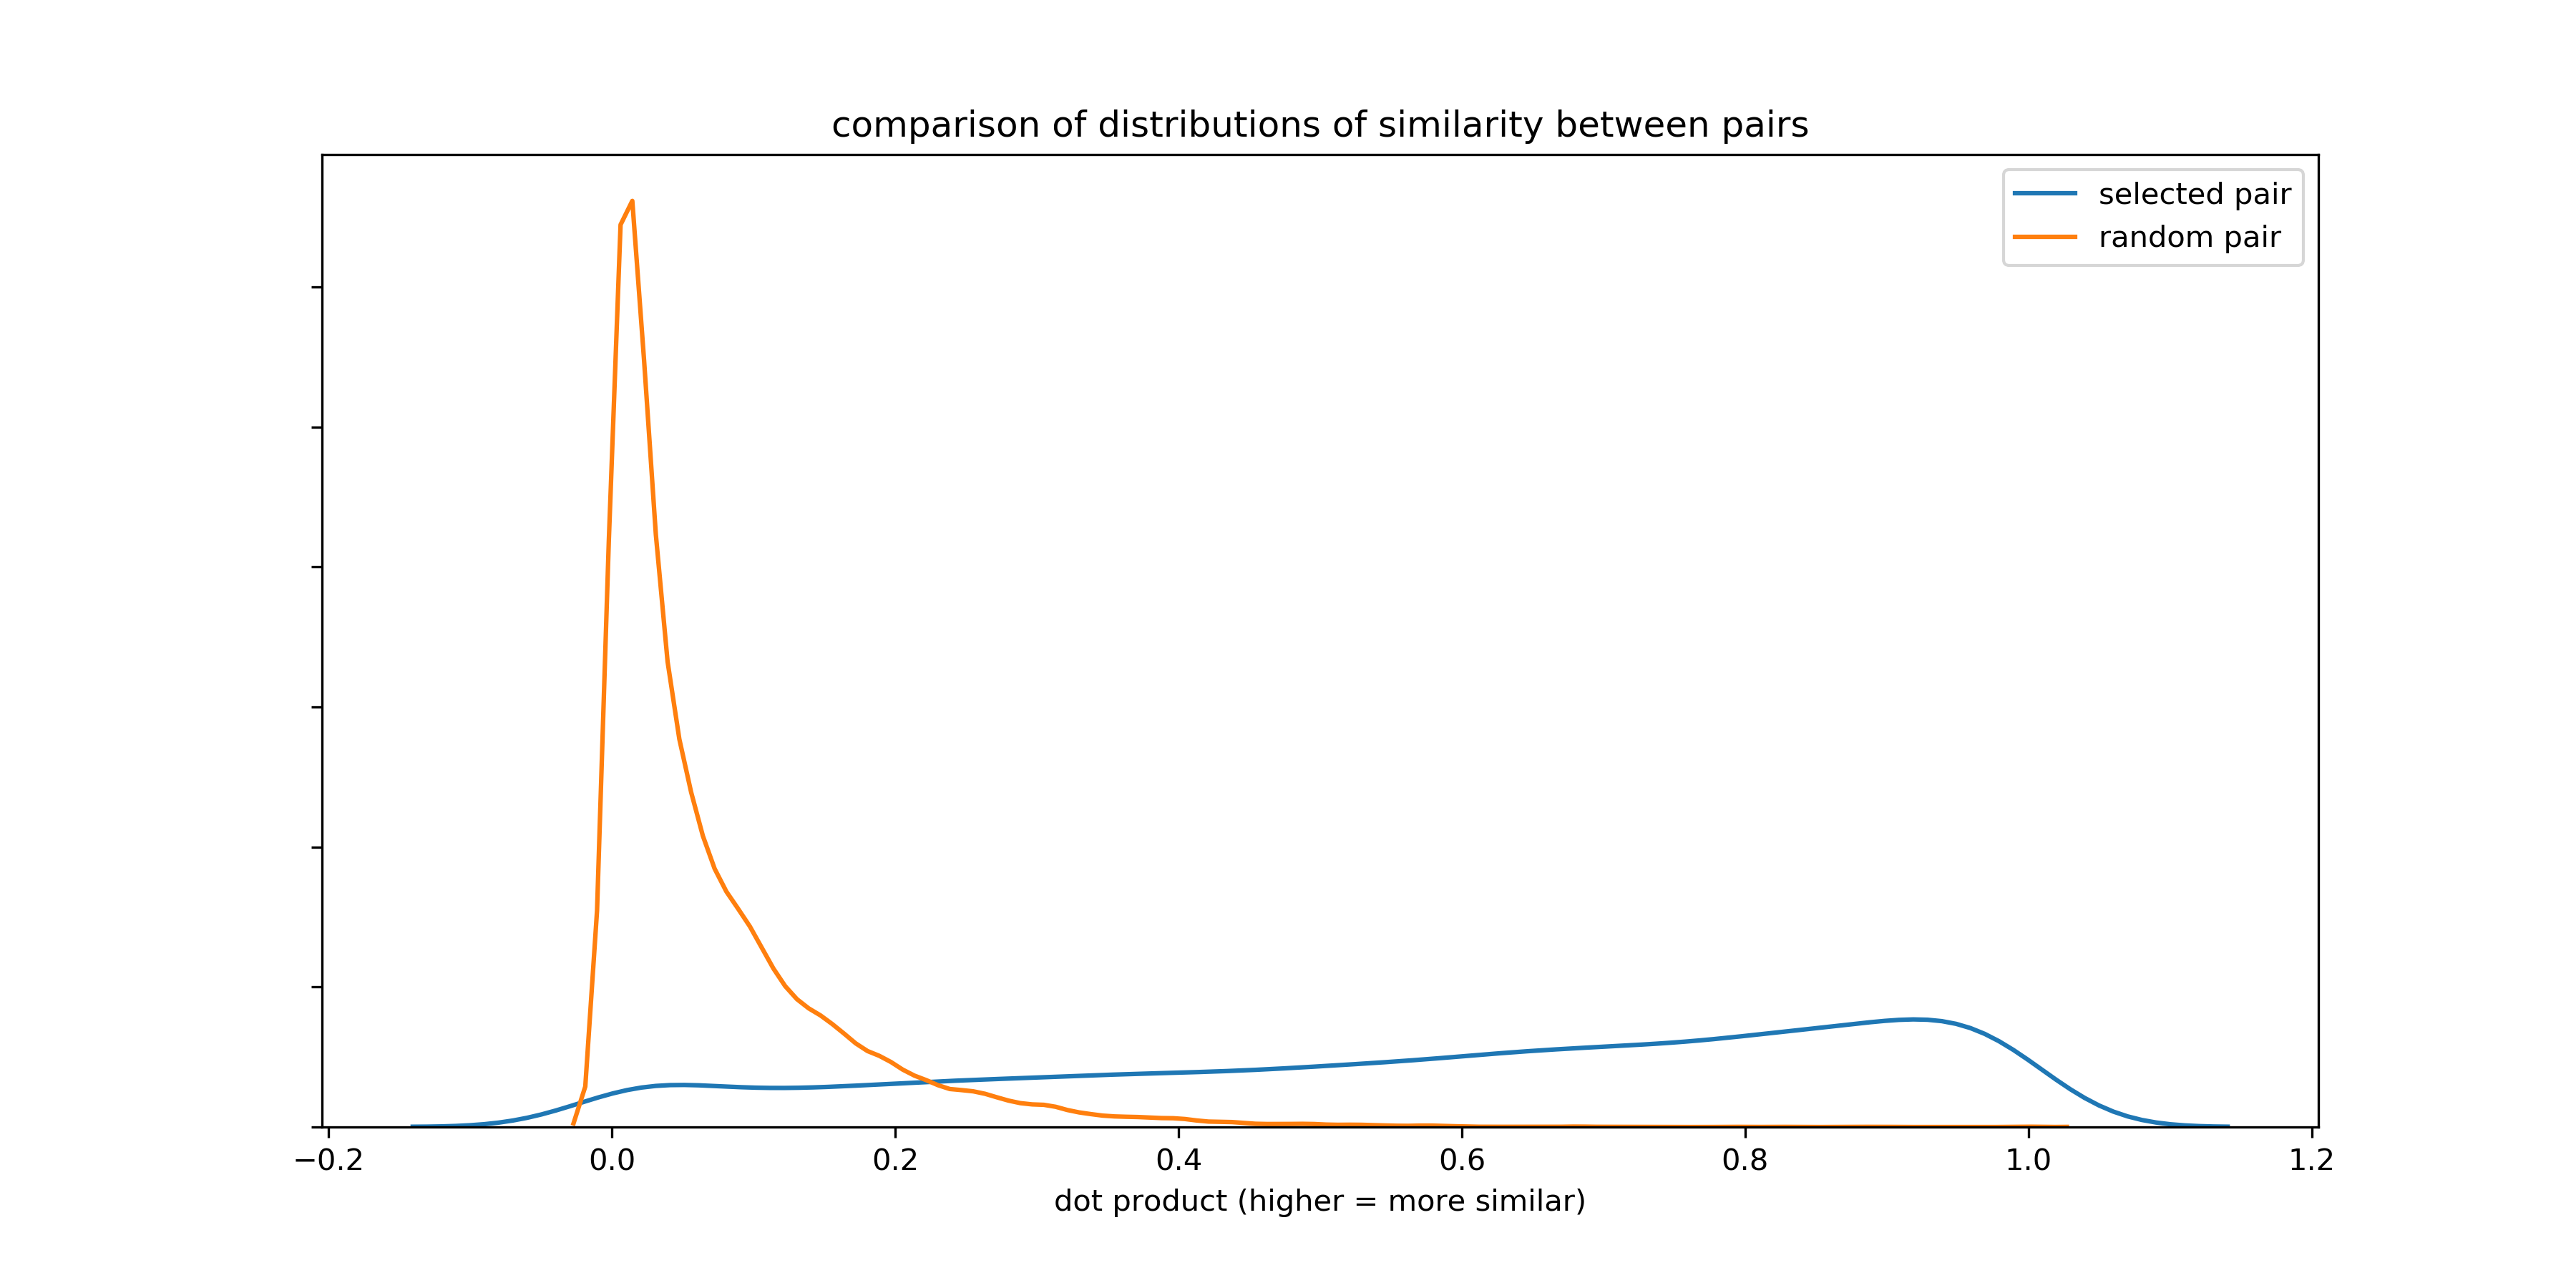
\includegraphics{pairs_comparison.png}
\caption{Evaluating equation pairs via equivalencies}
\end{figure}

One way to evaluate how useful this process of splitting on relations is
by checking the term-frequency-inverse-document-frequency similarity
scores between the pairs of equations, and comparing these scores with
randomly assigned pairs of equations. We would expect that equations
identified via equivalencies would have a pretty high similarity to each
other, on average, since people tend to repeat tokens on either side of
a relation (\(x + 6 = x + 3 + 3\), for example).

The histogram at the beginning of the section compares the similiarity
scores for the two across a sample of 100,000 equations. A higher score
on the x axis means equations are more similar.

You can see, based on this graph, that the probability of a pair of
equations identified through the methodology laid out in this report
being similar is much higher than that of a random pair.

\begin{figure}
\centering
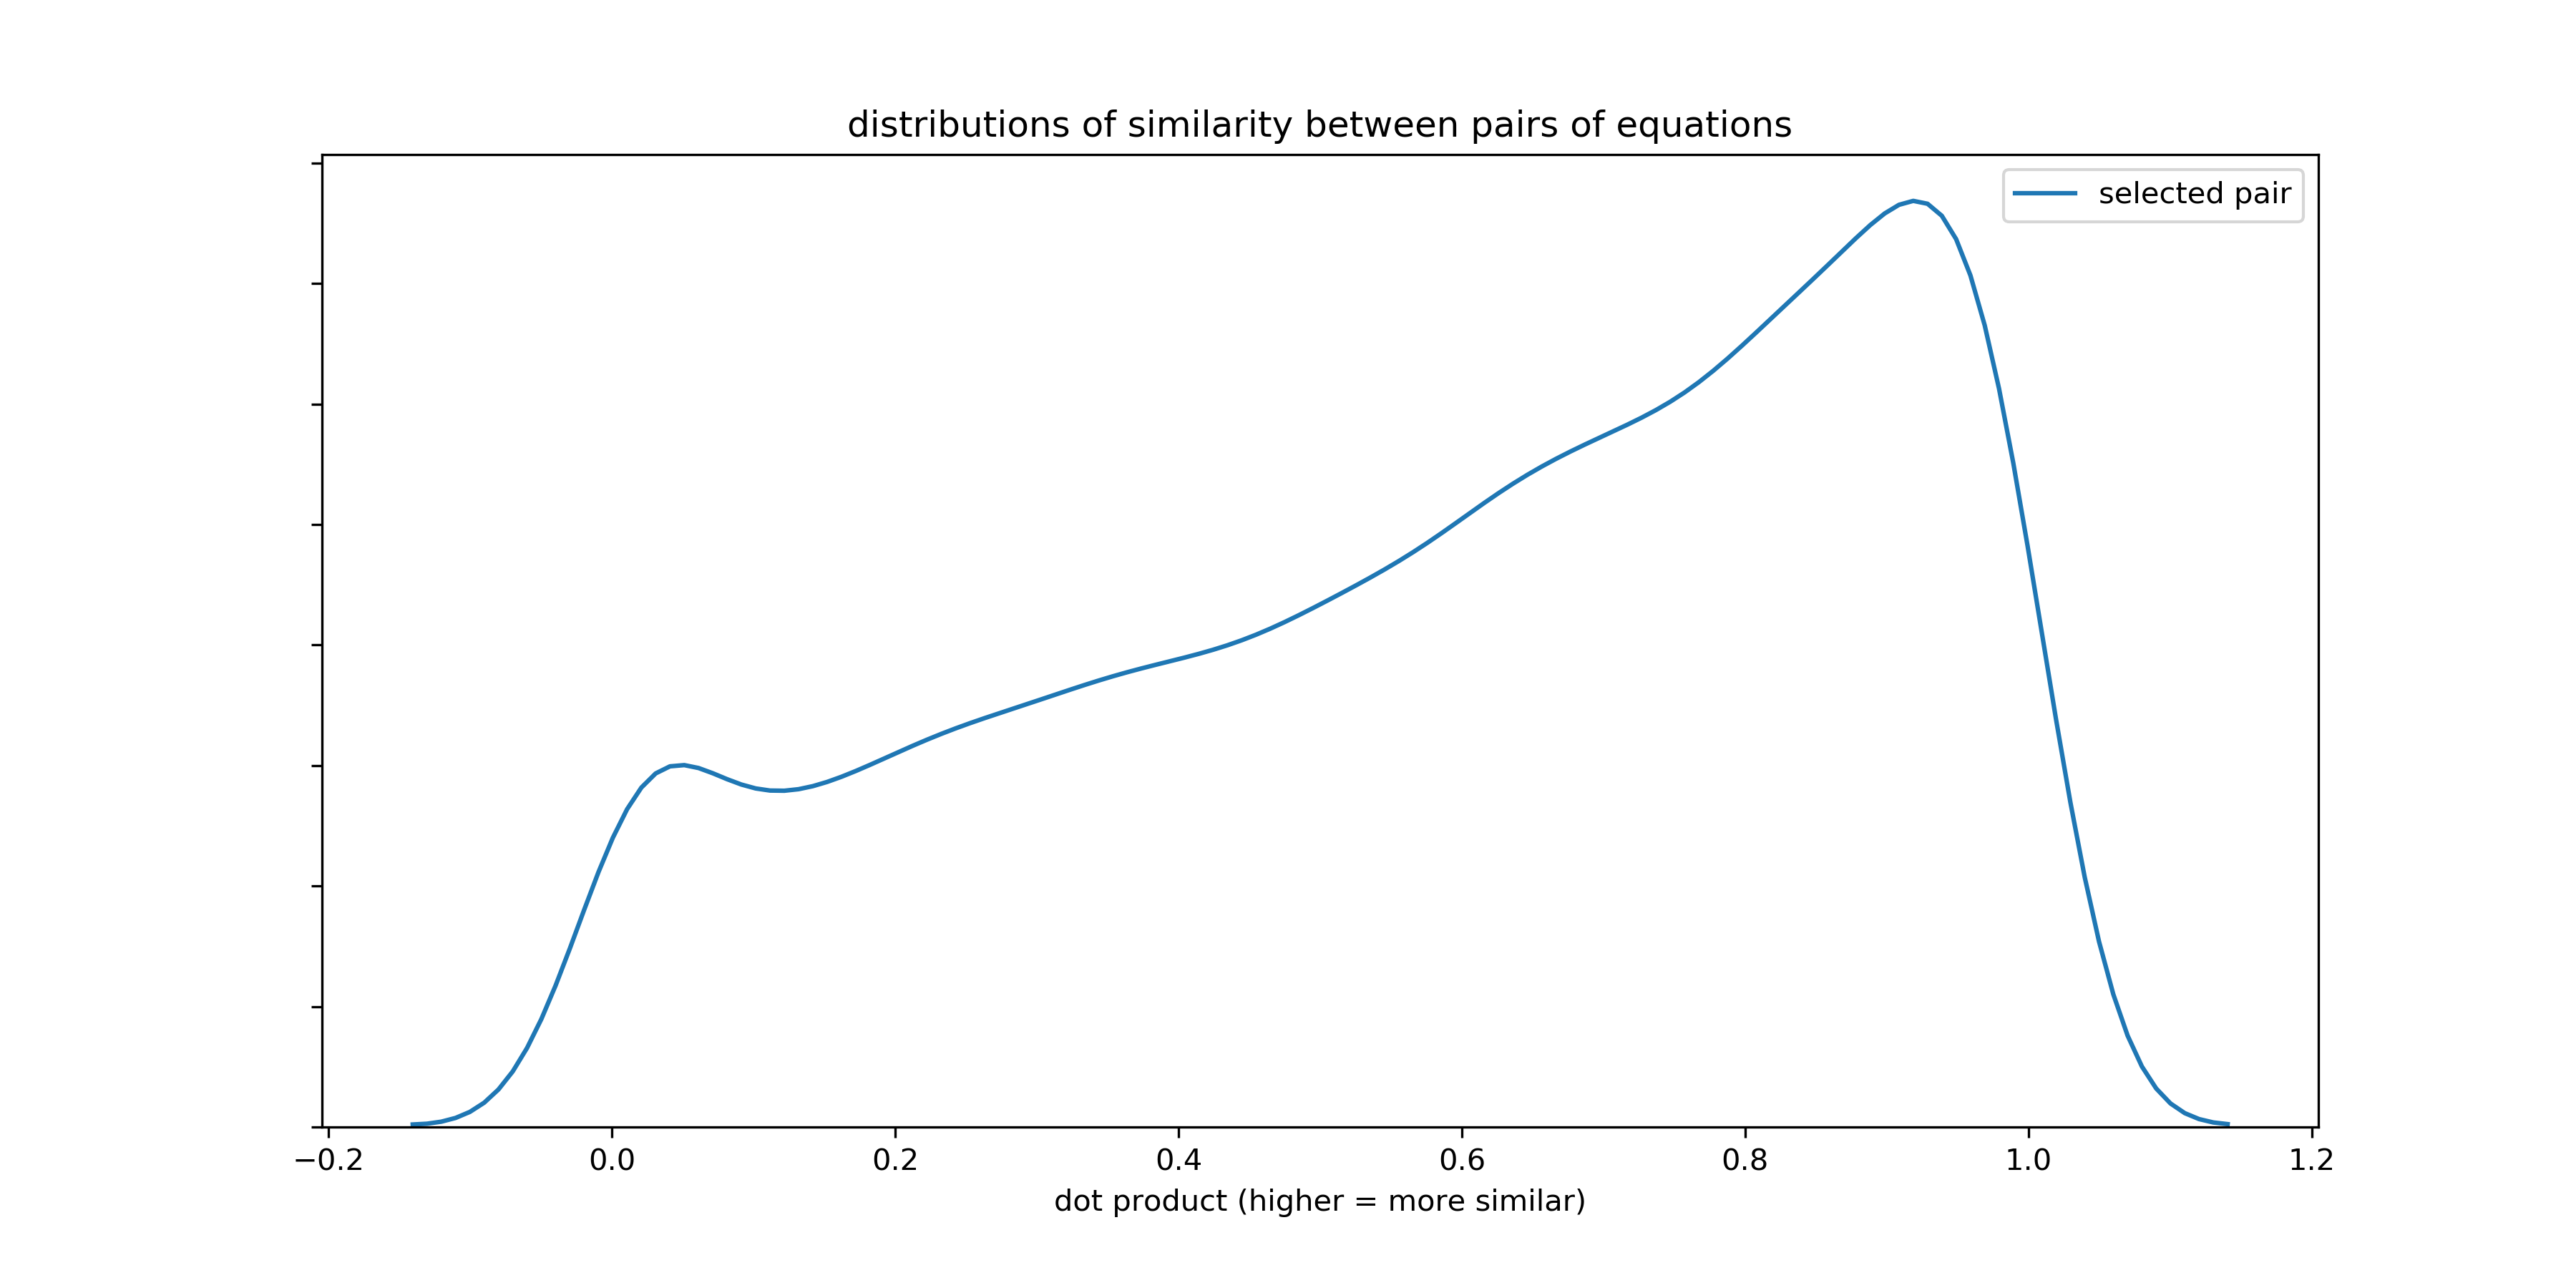
\includegraphics{pairs_dist.png}
\caption{Zooming in on the pairs}
\end{figure}

It is a bit hard to see what the distribution of pairs identified
through my methods is like since TF-IDF has such a higher peak. Plotted
alone, the graph is more or less normally distributed. This is
encouraging, since we would expect some sort of natural gradient to how
similar equation are, and yet also expect many to be very similar (but
not \emph{too} similar).

\hypertarget{bibliography}{%
\section*{Bibliography}\label{bibliography}}
\addcontentsline{toc}{section}{Bibliography}

\hypertarget{refs}{}
\leavevmode\hypertarget{ref-noauthor_neural_nodate}{}%
``A Neural Network for Machine Translation, at Production Scale.'' n.d.
\emph{Research Blog}. Accessed February 2, 2018.
\url{https://research.googleblog.com/2016/09/a-neural-network-for-machine.html}.

\leavevmode\hypertarget{ref-samghelms_mathviz:_2017}{}%
Helms, Samuel. 2017. ``Mathviz: A Python Package for Examining
Mathematics Equation Embeddings.'' https://github.com/samghelms/mathviz.

\leavevmode\hypertarget{ref-schnabel_evaluation_2015}{}%
Schnabel, Tobias, Igor Labutov, David Mimno, and Thorsten Joachims.
2015. ``Evaluation Methods for Unsupervised Word Embeddings.'' In,
298--307. \url{https://doi.org/10.18653/v1/D15-1036}.

\end{document}
